% Drawing 138/07-7 -- folder 138, batch 07, archive page 126 (PDF page 127).
% Transcription: une sphère avec équateur et méridien en pointillé, les points $0$, $1$, $\infty$ marqués ; deux petits triangles portant le graphe dual (un « Y » intérieur), l'un avec le sommet $0$ ; un losange coupé par une diagonale et un « Y ».
% Kind: sphere; triangles with dual graph; rhombus. Method 2 (schematic redraw from the facsimile). Status: ok.
% Notes: A sphere: its outline (one closed stroke), the equator in two strokes (the back half through the point infinity, the front half through 0 and 1, meeting at both ends inside the outline), the front meridian from the north point to the south point in two strokes broken at the equator, and the two back meridians as the dashes he drew, each dash a separate stroke (eight on the left, from the north point round to the bottom; nine on the right, two of them the small ticks beside the label 1); at the left, inside the outline, a second solid stroke above the equator and a short faint stroke outside it below. Points: north, south, 0 (front left), 1 (right), infinity (back). Labels 0, 1, infinity where he wrote them. Two triangles carrying the dual graph: in the first (hypotenuse faint, right side curved) a « Y » whose three arms end on the three sides; in the second, with the vertex 0 (no dot on the page), the « Y » drawn as the corner of a small square at the right angle plus an arm to the hypotenuse, with a small tick in the corner and an isolated dot below the right angle. A rhombus whose four sides are separate strokes as on the page (the upper left side thick; the lower sides do not reach the vertices), the horizontal diagonal in two pieces, the vertical diagonal in two pieces (broken below the centre, as on the page), and a thick « Y » centred where the upper vertical meets the horizontal. Second pass 2026-11-14 (issue 147, Claude Opus 5.5): redrawn stroke by stroke from grid overlays at 24 to 40 px per unit (the earlier redraw had the sphere as two ellipses about 2 units off, the back meridians as two long dashed arcs stopping at the equator, the triangles and the rhombus as polygons 1 to 2 units off, the vertical diagonal whole). The rasterised redraw laid over the crop: every stroke on its ink to within about half a unit. Not covered by this mark and not drawn: the triangle with a wavy curve at the lower left and the arc at the lower right (the next figure). Left out: the long faint lines crossing the region (a cone drawn across the page), and the formulas « 2z^2 - 2z = 0 », « z = ... ». Nothing is struck. Not compiled (no TeX engine in the session).
% Coordinates: 1 unit = 1 mm = 1/100 of the crop width (bbox in page fractions: [0.45, 0.355, 0.85, 0.54]).
% Redrawn by Claude (claude-opus-5-5), issue #73, 2026-11-09; not checked by a human; not compiled (no TeX in the session).
% Checked by Claude (claude-opus-5-5) 2026-11-14 (issue #147, second pass): strokes redrawn from the 300 dpi colour render of the 250 ppi scan, coordinates read on a grid overlay and checked by overlaying the rasterised redraw; not compiled (no TeX in the session). Not checked by a human. Status: ok.
% Rights: reproduces part of the work -- behind RENDER_TRANSCRIPTS, never published by itself.
\documentclass[tikz,border=3pt]{standalone}
\usepackage{amsmath,amssymb}
\usetikzlibrary{patterns,arrows.meta}
\tikzset{pencil/.style={black!45}, struck/.style={black!35}, mark/.style={circle,draw,inner sep=1.3pt}, pt/.style={circle,fill,inner sep=0.9pt}, opt/.style={circle,draw,fill=white,inner sep=1.1pt}}
\begin{document}
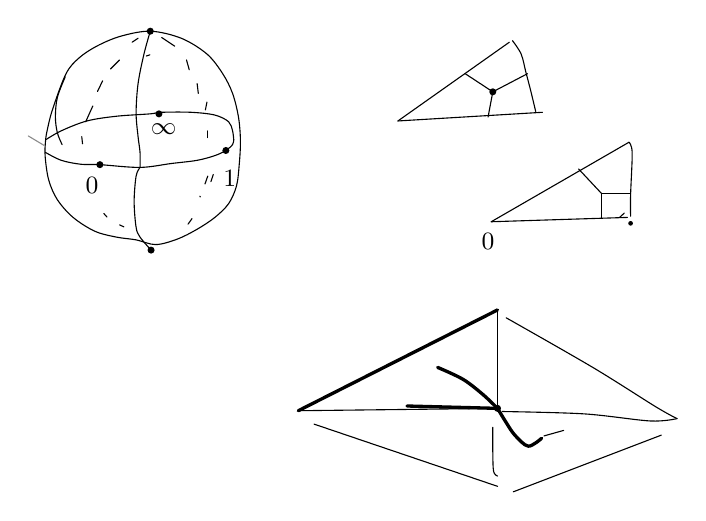
\begin{tikzpicture}[x=1mm,y=1mm,line cap=round,line join=round,font=\scriptsize]
\draw plot[smooth cycle, tension=0.55] coordinates {(24.3,-5.1) (28.25,-6) (31.5,-8) (33.5,-10.5) (34.75,-13) (35.5,-16) (35.75,-19) (35.6,-22) (35.25,-24.75) (34.25,-27) (32.5,-28.75) (30.25,-30.25) (27.75,-31.5) (25,-32.2) (22.5,-31.6) (20,-31.25) (17.25,-30.5) (14.5,-28.75) (12.5,-26.5) (11.4,-24) (10.95,-21) (11,-19) (11.25,-17.5) (11.9,-15) (13.6,-10.5) (15.25,-8.5) (17.5,-7) (20.5,-5.75)};
\draw plot[smooth, tension=0.55] coordinates {(13.5,-10.9) (12.5,-13.5) (12.25,-16) (12.5,-18) (13.1,-19.5)};
\draw[pencil] (8.8,-18.4) -- (10.8,-19.6);
\draw plot[smooth, tension=0.55] coordinates {(11,-18.9) (13,-17.75) (16.25,-16.5) (20,-15.9) (24.25,-15.6) (25.75,-15.4) (29.5,-15.4) (32.5,-15.75) (34.25,-16.6) (34.75,-17.75) (34.9,-18.9)};
\draw plot[smooth, tension=0.55] coordinates {(11,-20.5) (13,-21.5) (15.5,-22) (17.9,-22.05) (23,-22.4) (27,-21.9) (30.25,-21.5) (32.5,-20.9) (33.9,-20.25) (34.75,-19.5) (34.9,-18.9)};
\draw plot[smooth, tension=0.55] coordinates {(24.3,-5.1) (23.5,-8) (22.75,-11.75) (22.5,-15.5) (22.75,-18.5) (23,-20.5) (23,-22.4)};
\draw plot[smooth, tension=0.55] coordinates {(23,-22.4) (22.5,-23.5) (22.25,-26.75) (22.5,-30) (23,-31.25) (24.4,-32.9)};
\draw (22,-6.5) -- (22.75,-6);
\draw (23.8,-8.25) -- (24.25,-8.1);
\draw (19.25,-9.9) -- (20.4,-8.75);
\draw (17.6,-12.75) -- (18.25,-11.4);
\draw (16.1,-16.6) -- (17,-14.6);
\draw (15.6,-18.5) -- (15.7,-19.4);
\draw (18.4,-28.25) -- (18.8,-28.7);
\draw (20.4,-29.7) -- (20.95,-29.95);
\draw (25.75,-5.9) -- (27.4,-7);
\draw (28.9,-8.75) -- (29.25,-10);
\draw (30.25,-11.75) -- (30.4,-13);
\draw (31.5,-14.1) -- (31.3,-15.1);
\draw (31.6,-17.75) -- (31.6,-18.6);
\draw (31.25,-24.5) -- (31.6,-23.5);
\draw (32,-24.2) -- (32.3,-23.3);
\draw (30.6,-26.05) -- (30.65,-26.15);
\draw (29.1,-29.6) -- (29.6,-28.9);
\node[pt] at (24.3,-5.1) {};
\node[pt] at (24.4,-32.9) {};
\node[pt] at (17.9,-22.05) {};
\node[pt] at (33.9,-20.25) {};
\node[pt] at (25.4,-15.6) {};
\node[inner sep=1pt] at (16.9,-24.75) {\small $0$};
\node[inner sep=1pt] at (34.4,-23.8) {\small $1$};
\node[inner sep=1pt] at (26,-17.5) {\small $\infty$};
\draw (55.75,-16.5) -- (69.9,-6.5);
\draw plot[smooth, tension=0.55] coordinates {(70.3,-6.3) (71.4,-8) (72,-10.3) (72.6,-12.6) (73.25,-15.3)};
\draw (55.75,-16.5) -- (74.1,-15.4);
\draw (67.8,-12.8) -- (64.3,-10.5);
\draw (67.8,-12.8) -- (72.2,-10.5);
\draw (67.8,-12.8) -- (67.2,-16);
\node[pt] at (67.8,-12.8) {};
\draw (67.6,-29.3) -- (85.1,-19.2);
\draw plot[smooth, tension=0.55] coordinates {(85.1,-19.2) (85.5,-20.5) (85.3,-25.9) (85.3,-28.6)};
\draw (67.6,-29.3) -- (84.9,-28.75);
\draw (78.7,-22.6) -- (81.6,-25.7);
\draw (81.6,-25.7) -- (85.3,-25.7);
\draw (81.6,-25.7) -- (81.6,-28.8);
\draw (83.9,-28.75) -- (84.5,-28.2);
\fill (85.3,-29.5) circle[radius=0.3];
\node[inner sep=1pt] at (67.2,-31.75) {\small $0$};
\draw[very thick] (43.1,-53.3) -- (68.4,-40.5);
\draw plot[smooth, tension=0.55] coordinates {(69.5,-41.5) (80.5,-47.8) (88.5,-52.8) (91.2,-54.3)};
\draw (45.1,-55) -- (68.4,-62.9);
\draw (70.4,-63.6) -- (89.2,-56.4);
\draw (43.1,-53.3) -- (68.4,-53);
\draw plot[smooth, tension=0.55] coordinates {(69,-53.4) (79.4,-53.7) (87.8,-54.6) (91.2,-54.3)};
\draw (68.4,-40.5) -- (68.4,-53);
\draw plot[smooth, tension=0.55] coordinates {(67.8,-55.4) (67.8,-58.5) (67.9,-61) (68.4,-61.6)};
\draw[very thick] plot[smooth, tension=0.55] coordinates {(60.8,-47.8) (64,-49.3) (66.5,-51.2) (68.4,-53)};
\draw[very thick] (56.9,-52.7) -- (68.4,-53);
\draw[very thick] plot[smooth, tension=0.55] coordinates {(68.4,-53) (69.5,-54.8) (70.6,-56.4) (72.3,-57.8) (74,-56.8)};
\draw (74.3,-56.5) -- (76.8,-55.8);
\node[pt] at (68.4,-53) {};
\end{tikzpicture}
\end{document}
